\documentclass{sigchi}

% Use this section to set the ACM copyright statement (e.g. for
% preprints).  Consult the conference website for the camera-ready
% copyright statement.

% Copyright
\CopyrightYear{2020}
%\setcopyright{acmcopyright}
\setcopyright{acmlicensed}
%\setcopyright{rightsretained}
%\setcopyright{usgov}
%\setcopyright{usgovmixed}
%\setcopyright{cagov}
%\setcopyright{cagovmixed}
% DOI
\doi{https://doi.org/10.1145/3313831.XXXXXXX}
% ISBN
\isbn{978-1-4503-6708-0/20/04}
%Conference
\conferenceinfo{CHI'20,}{April  25--30, 2020, Honolulu, HI, USA}
%Price
\acmPrice{\$15.00}

% Use this command to override the default ACM copyright statement
% (e.g. for preprints).  Consult the conference website for the
% camera-ready copyright statement.

%% HOW TO OVERRIDE THE DEFAULT COPYRIGHT STRIP --
%% Please note you need to make sure the copy for your specific
%% license is used here!
% \toappear{
% Permission to make digital or hard copies of all or part of this work
% for personal or classroom use is granted without fee provided that
% copies are not made or distributed for profit or commercial advantage
% and that copies bear this notice and the full citation on the first
% page. Copyrights for components of this work owned by others than ACM
% must be honored. Abstracting with credit is permitted. To copy
% otherwise, or republish, to post on servers or to redistribute to
% lists, requires prior specific permission and/or a fee. Request
% permissions from \href{mailto:Permissions@acm.org}{Permissions@acm.org}. \\
% \emph{CHI '16},  May 07--12, 2016, San Jose, CA, USA \\
% ACM xxx-x-xxxx-xxxx-x/xx/xx\ldots \$15.00 \\
% DOI: \url{http://dx.doi.org/xx.xxxx/xxxxxxx.xxxxxxx}
% }

% Arabic page numbers for submission.  Remove this line to eliminate
% page numbers for the camera ready copy
% \pagenumbering{arabic}

% Load basic packages
\usepackage{balance}       % to better equalize the last page
\usepackage{graphics}      % for EPS, load graphicx instead 
\usepackage[T1]{fontenc}   % for umlauts and other diaeresis
\usepackage{txfonts}
\usepackage{mathptmx}
\usepackage[pdflang={en-US},pdftex]{hyperref}
\usepackage{color}
\usepackage{booktabs}
\usepackage{textcomp}

% Some optional stuff you might like/need.
\usepackage{microtype}        % Improved Tracking and Kerning
% \usepackage[all]{hypcap}    % Fixes bug in hyperref caption linking
\usepackage{ccicons}          % Cite your images correctly!
% \usepackage[utf8]{inputenc} % for a UTF8 editor only

% If you want to use todo notes, marginpars etc. during creation of
% your draft document, you have to enable the "chi_draft" option for
% the document class. To do this, change the very first line to:
% "\documentclass[chi_draft]{sigchi}". You can then place todo notes
% by using the "\todo{...}"  command. Make sure to disable the draft
% option again before submitting your final document.
\usepackage{todonotes}

% Paper metadata (use plain text, for PDF inclusion and later
% re-using, if desired).  Use \emtpyauthor when submitting for review
% so you remain anonymous.
\def\plaintitle{Plexus: Guiding Novice Transport Planners through Expert-authored Data Stories}
\def\plainauthor{Allyza Mae Acu\~na, Krizia Lynn Chiu, Louise Anne Cortez, Sophia Therese Rivera, Rafael Cabredo, Briane Paul Samson}
\def\emptyauthor{}
\def\plainkeywords{Transport planning; Spatial analysis and interpretation; novice transport planners;co-design}
\def\plaingeneralterms{Documentation, Standardization}

% llt: Define a global style for URLs, rather that the default one
\makeatletter
\def\url@leostyle{%
  \@ifundefined{selectfont}{
    \def\UrlFont{\sf}
  }{
    \def\UrlFont{\small\bf\ttfamily}
  }}
\makeatother
\urlstyle{leo}

% To make various LaTeX processors do the right thing with page size.
\def\pprw{8.5in}
\def\pprh{11in}
\special{papersize=\pprw,\pprh}
\setlength{\paperwidth}{\pprw}
\setlength{\paperheight}{\pprh}
\setlength{\pdfpagewidth}{\pprw}
\setlength{\pdfpageheight}{\pprh}

% Make sure hyperref comes last of your loaded packages, to give it a
% fighting chance of not being over-written, since its job is to
% redefine many LaTeX commands.
\definecolor{linkColor}{RGB}{6,125,233}
\hypersetup{%
  pdftitle={\plaintitle},
% Use \plainauthor for final version.
%  pdfauthor={\plainauthor},
  pdfauthor={\emptyauthor},
  pdfkeywords={\plainkeywords},
  pdfdisplaydoctitle=true, % For Accessibility
  bookmarksnumbered,
  pdfstartview={FitH},
  colorlinks,
  citecolor=black,
  filecolor=black,
  linkcolor=black,
  urlcolor=linkColor,
  breaklinks=true,
  hypertexnames=false
}

% create a shortcut to typeset table headings
% \newcommand\tabhead[1]{\small\textbf{#1}}

% End of preamble. Here it comes the document.
\begin{document}

\title{\plaintitle}

\numberofauthors{3}
\author{
  \alignauthor{Allyza Mae Acu\~na\\
    \affaddr{De La Salle University}\\
    \affaddr{Manila, Philippines}\\
    \email{allyza\_acuna@dlsu.edu.ph}}\\
  \alignauthor{Krizia Lynn Chiu\\
    \affaddr{De La Salle University}\\
    \affaddr{Manila, Philippines}\\
    \email{krizia\_chiu@dlsu.edu.ph}}\\
  \alignauthor{Louise Anne Cortez\\
    \affaddr{De La Salle University}\\
    \affaddr{Manila, Philippines}\\
    \email{louise\_cortez@dlsu.edu.ph}}\\
\alignauthor{Sophia Therese Rivera\\
    \affaddr{De La Salle University}\\
    \affaddr{Manila, Philippines}\\
    \email{sophia\_rivera@dlsu.edu.ph}}\\
\alignauthor{Rafael A. Cabredo\\
    \affaddr{De La Salle University}\\
    \affaddr{Manila, Philippines}\\
    \email{rafael.cabredo@dlsu.edu.ph}}\\
\alignauthor{Briane Paul V. Samson\\
    \affaddr{Future University Hakodate}\\
    \affaddr{Hakodate, Japan}\\
    \affaddr{De La Salle University}\\
    \affaddr{Manila, Philippines}\\
    \email{briane.samson@dlsu.edu.ph}}\\
}
\maketitle

\begin{abstract}
  To create data-driven decisions, formal knowledge and utilization of decision support systems is recommended. Therefore, transport planning processes are ideally implemented by trained engineers within a government unit to make decisions regarding land-use and transport. However, local government units at present lack resources to acquire transport planning tools and to hire formally trained engineers. Current tools need expert knowledge and training; Providing them just exploratory tools might not always transfer expertise or support effective assessments and planning. Through identifying the workflow patterns of engineers and the mental models of novices using co-design, we created Plexus, a web application designed to aid novices in transport desirability assessment using expert-authored data stories. To evaluate the effectiveness of the expert-authored data stories in transferring knowledge, an expert will assess the outputs from participants who used only Excel files, a Plexus version without data stories, and a Plexus version with data stories.
\end{abstract}


% ACM Classfication

 \begin{CCSXML}
<ccs2012>
<concept>
<concept_id>10003120.10003123.10010860.10010859</concept_id>
<concept_desc>Human-centered computing~User centered design</concept_desc>
<concept_significance>500</concept_significance>
</concept>
</ccs2012>
\end{CCSXML}

\ccsdesc[500]{Human-centered computing~User centered design}
\ccsdesc[500]{Human-centered computing~Human computer interaction (HCI)}
\ccsdesc[100]{Human-centered computing~User studies}

% Author Keywords
\keywords{\plainkeywords}

% Print the classficiation codes
\printccsdesc
% Please use the 2012 Classifiers and see this link to embed them in the text: \url{https://dl.acm.org/ccs/ccs_flat.cfm}



\section{Introduction}

Transport planning is a cooperative process that requires the involvement of stakeholders to strategize operation, maintenance, and management of an area's transport system to meet the area's long-term goals. The effects of urbanization could also be endured in areas through transport planning, as it is the process of studying the current state of certain areas and finding strategic ways on how to solve problems encountered in them \cite{Palma2017}, ranging from environmental management to transportation. It is also a complex analytical and cyclical process of balancing multiple decision criteria from a range of factors \cite{Simao2009}.

In order to make good decisions regarding infrastructure, zoning, and routing, formal knowledge in transport engineering and transport-related decision-support systems are currently used to make data-driven assessments. However, the lack of transport planning education has caused developing countries to barely endure rapid urbanization \cite{evren2001transportation}. Additionally, the lack of integrated planning across transport modes and land use, conflicting government policies at local and national levels, misaligned plans, and lack of funds have led  to developing countries having poor transport infrastructure \cite{mahendra2016,gwilliam1999public}. In the context of the Philippines, there is an imbalance in the development of urban planning divisions between local government units (LGUs). Although a comprehensive land-use plan (CLUP) is currently utilized by Philippine cities and municipalities, departments officials for transport planning or transport management are not required to have formal training in such. Moreover, officials are also not required to have knowledge in systems that aid in transport planning, as most government units cannot afford to acquire such systems.  

A challenge in making transport-related decisions is to create assessments to support these. Experts, who are formally trained in transport engineering, utilize tools and their knowledge on transportation-related theories and concepts to have data-driven assessments. Moreover, formal training is required before using these tools as they are only catered to expert users. These tools only provide features for users to decide on relevant information for them, and not necessarily guiding them to create an assessment. Also, there are multiple visualizations and data available within the system, which could overwhelm novice users. While experts have patterns to create quality transport-related assessments using these tools, novices may not have background on transport engineering concepts in theories, leading to them miss important information. Moreover, even if a novice captures the right types of information, the information may not be used effectively to achieve important insights.

In this study, we devised a co-design approach to guide novices to make assessments through transferring expert knowledge. We hypothesized that if we have data summaries and helpful interactions within our system, we can guide novices to create transport-related assessments. We used the transport desirability framework, which shows how desirable an area is based on accessibility of amenities and transport modes, travel cost and travel time, and the experiences of residents during flooding and using transportation. This framework served as the basis for resulting assessments from the system. We conducted co-design sessions with LGU planning and management officials and transport engineer researchers to find workflow and important information and visualizations for assessment. Using insights from these sessions, we created a prototype of our proposed system, Plexus, and continued refining it through multiple iterations of usability testing. After these multiple evaluations, we resulted with a web application that comprises of an interactive map and data summaries containing explanatory data. 

To test if our hypothesis is true, we will be conducting an experiment wherein novices will be using different tools, including Plexus with data stories, to make assessments. Resulting assessments will be rated by a transport desirability expert to conclude if assessments had better quality when using the tool with data stories. 

\section{Related Work}

\subsection{Data Stories}
Data stories are a combination of narratives and interactive or static data visualizations \cite{Segel2011}. Usually, data visualizations provide supporting or related details to the narrative. Narratives are presented in a meaningful order to communicate ideas from the author to the readers, which can be called author-driven \cite{Lee2015}. However, the arrangement of these narratives could also be reader-driven, wherein there is no strict order of information and a high degree of interactivity \cite{Segel2011}. Choosing between these two approaches depends on the complexity of the data and narrative, and the intended audience. Utilizing messaging to explain ideas and data visualizations may clarify the narrative, but might clutter the interface. On the other hand, interactivity may engage user exploration, but might not lead to the intended message of the author. 

There has been an ongoing discussion about data stories being beneficial. Multiple studies have concluded that data stories were seen as a powerful way to summarize various information, to subtly explore data, to discover new questions about the data, and to deliver ideas or messages to the readers \cite{Pavel2013} \cite{Layton2014}. FinaVistory used data stories to help readers understand financial news \cite{Chan2016}; However, the data stories were interactive, allowing users to choose what to focus on. In MeetingVis, data stories were effective in memory retrieval for meetings through showing essential meeting elements \cite{Shi2018}. Other than interactivity, tooltips and backstories to clarify context were considered beneficial by Figueiras \cite{Figueiras2014}. This is supported in the study of GameFlow, which stated that although users were satisfied with the visualizations, textual narrations to complement the visualizations were suggested \cite{Chen2016}. Although these studies curated data stories, stakeholder participation in design and in evaluation was not prioritized. Moreover, evaluation was feature-based and not focused on the effect on understanding messages. Therefore, our study aims to contribute by incorporating co-design in creating the application and evaluation of resulting assessments through data stories. 

\subsection{Current transport planning-related tools}

Current tools for transport planning and other related processes usually have travel demand forecasting models, cost-benefit analysis, statistical graphs, simulations, and multiple interactive visualizations. Some tools that are utilized for transport planning are QGIS, EMME, Cube, JICA Strada, and Visum. A common feature of these systems is that all have visualizations for statistical analysis and other supporting data superimposed on map visualizations. Moreover, users are given the option to analyze raw quantities through a table instead of a visualization. Choropleth maps are not usually used in these systems; Therefore, these systems are used to model traffic or transport patterns, and are not focused on area-based household data and travel data. Moreover, since there are multiple options to visualize and use data for calculations, one must have formal training in order to utilize these systems effectively. Novices will most likely be overwhelmed by the amount of possibilities that could be done within the systems, leading to the inability to maximize the insights they could gather.

\subsection{Novice Support Tools}
Novice support tools have simplified interfaces and limited functions to lessen the cognitive load of users. These tools are created to make difficult tasks, usually requiring expert knowledge, easier for novices. Moreover, these  tools are created to ease the difficulty of learning a skill or a process. DrawMyPhoto is an example of a tool that focused on simplifying interfaces by removing grids and limited functions by removing manually chosen stroke width, color, and darkness \cite{Williford2019}. The system also adopts techniques from experts by using light blue color for reference images, which is a popular underlay color in architectural drafting. Motif is another tool that supports novices to create expert-like outputs using expert patterns that novices need to follow \cite{Kim2015}. Other than these studies, other related studies are evaluated through an expert assessing the outputs of novices. In the case of both Motif and DrawMyPhoto, the studies achieved positive results in supporting novices with achieving difficult tasks.  
\subsection{Co-design}
To ensure the effectiveness of a tool being developed, studies posit that involving end-users and consultants early on in the design process is a beneficial step. Co-design supports discussion with end-users, consultants, and  proponents regarding the design of the interface, features, and workflow of the tool. For SpeechBubbles, multiple interviews were done with end-users to understand their situation and pain points. After analyzing the pain points of the participants, they were asked to design visualizations and suggest features with other participants \cite{Peng2018}. Insights from the session led to the creation of the prototype, which was refined through multiple design critiques with co-design participants. Another study used co-design on low-tech prototyping, and involved groups of children, teachers, and HCI experts \cite{Alhumaidan2015}. Using co-design reveals the challenges faced by each stakeholder, which leads to proponents adjusting workflow, interface, and features in the tool as early as possible. 

\section{Co-design of Plexus}

\subsection{First co-design session}
The first was done to identify the expectations of novices and subject-matter experts when creating transport assessments; Expectations that were gathered were about the steps in using the application, and the visualizations and the data they expect to utilize. This session had 5 local government officials under the department of planning or transport management and 1 subject-matter expert who was a transport engineer. 

\subsection{Insights}
\subsubsection{Strategies for decision-making are trial-and-error}
From the co-design session, an eminent theme was the insufficiency of data and resources for transport planning. Varying processes in transport planning have elicited different results from LGUs with regard to their process. However, officials from both cities base their decisions on observations or assumptions of the current traffic situation and socioeconomic and vehicle count data. These decisions, however, are evaluated based on the degree of traffic congestion observed in the area and are not based on commuter opinions or recorded data. 

\subsubsection{Tools to aid in transport planning are not used or are difficult to use}
Aside from the lack of a centralized process, LGU officials have mentioned that they do not use any tool to help them in their tasks, and instead rely on non-visualized data and observations of the area. Although they use maps for observing the land-use in the area, they do not use other visualizations besides choropleth maps. Additionally, according to transport engineers, current systems such as EMME are difficult to use without prior training.  

\subsubsection{Most participants lack useful data and visualizations}
In line with this, data from commuters are significantly deficient as LGU officials have mentioned wanting to be knowledgeable about commuters’ opinions on changes in public transport. As officials do not have access to more information regarding transport and commuter behavior, the current process results to decisions in their city being tested through trial and error. Apart from this, accessible data is usually presented in figures and may not be aggregated.

Due to this issue, officials expect that they would make more informed transport decisions when given more and well-presented data. Data stated to be useful include origin and destination points, spatial amenities in the area, and economic and temporal indicators from the transport desirability framework. From this, they also mapped visualizations that they think would assist them in assessing transport in their respective cities. Choropleth maps were said to be understandable for representing indicators per barangay, lines and arcs were appropriate for origin and destination points and volume of commuters for a path, and icon maps were stated to be used to visualize amenities. Other visualizations such as hexagon binning and heatmaps were not utilized by the stakeholders.

\subsection{Second Co-design Session}
The second session was to identify data that would be beneficial in assessing each transport desirability indicator. This session had 2 transport desirability experts participate through cardsorting lists that were initially made using the first session insights. The cards consisted of the data, their visualizations, and the order of how this data will be presented to the user.

\subsection{Insights}
\subsubsection{General Information}
Demographic data, overall modeshare, and modeshare per barangay were deemed as important information and should be present when viewing any indicator or transport desirability. An indicator breakdown was also suggested to promote a top-down analysis. Land area, amenities, and origin-destination data were also considered as important information in assessing barangays, which are areas that are smaller than towns or cities. 

\subsubsection{Transport Desirability}
The co-design session resulted to three groups of information that LGUs believed would be useful to users. These groups are namely: 1) Route Development, 2) Mode Shift, and 3) Flooding. 

For information related to routes, origin-destination data along with their corresponding distances, travel costs, volume, and travel time, and mode share of the barangay was suggested by the experts. It would also be ideal for users to filter these information through demographics. Under Mode Shift, average comfort per transport mode, mode share by demographic, breaking down an origin-destination pair by mode share, health contribution per transport mode, travel time and travel cost per transport mode was suggested. Lastly, information that would be used to assess barangays and the city/town with regard to flooding were origin-destination pairs most affected by flood, survey results on how much a trip is affected by flood, range of travel cost and additional travel costs, range of travel time and additional travel time, energy use of transport mode, efficiency of per transport mode, and route and mode options during heavy rain and flooding. 

\subsubsection{Indicators}
Economic and temporal indicators would require the average, maximum, and minimum travel cost and travel time, top 10 and bottom 10 travel cost and travel time, cost and time to and from one barangay to another for public and private transport mode, mode share, amenities, and income distribution to assess properly. Data suggested for deeper assessment of the physical indicator would be the effect on commuters in terms of the percentage of people who are flooded along with their origin-destination pair, average, maximum, and minimum cost of commuters with their origin-destination pairs. A link to amenities and the answers to flood-related survey questions presented as a bar graph were also deemed useful. For the spatial indicator, it would be beneficial to present the accessibility of different income levels depending on their travel allowance, a breakdown count of per amenity, and a list of amenities that are reachable from a certain distance or time. For transport mode indicators, each would be linked to the physical indicator and spatial indicator as they were deemed useful.

\section{Designing Plexus}
Plexus is a visual analytics system that aims to aid novice users attain expert-like transport desirability assessments through interactive elements and data stories. Specifically, the system allows users to view and visualize cities' and barangays' transport desirability and transport desirability-related factors. It first directs the user to the home screen, where the list of available cities are presented to the user. Upon selecting a city from the Plexus home screen, the user would be directed to the assessment screen, containing various interactive elements: the map, the left side panel containing the city overview, the right side panel containing indicator overviews or barangay overviews, and the collapsed bottom panel containing data stories. Through the combined use of these various elements, the users could be aided with the transport assessment of the city.

We conducted four usability tests to refine system features and interface. The first usability test (UT1) included three novices from Metro Manila local government units (LGUs) who were part of the planning or transport management department and did not have any formal training in transport engineering and its tools (UT1N). Three experts (UT1E), who specialized in transport desirability assessment or transport engineering, were also included in the first usability test. The second usability test (UT2) included six novices who were knowledgeable in engineering concepts (UT2NN) and three novices who participated in the previous test (UT2FN). Two experts (UT2E) from the first usability test were invited again to participate in the second iteration. The third usability test (UT3) had three novices from Provincial local government units (UT3N) to test if the system would still be usable for them even if we co-designed with only Metro Manila LGUs. Finally, the fourth usability test (UT4) had two new experts (UT4E), who specialized in transport engineering, test the system to check the usability of the system for a trained eye.

\subsection{Exploring the Interactive Map}

\begin{figure}
\centering
  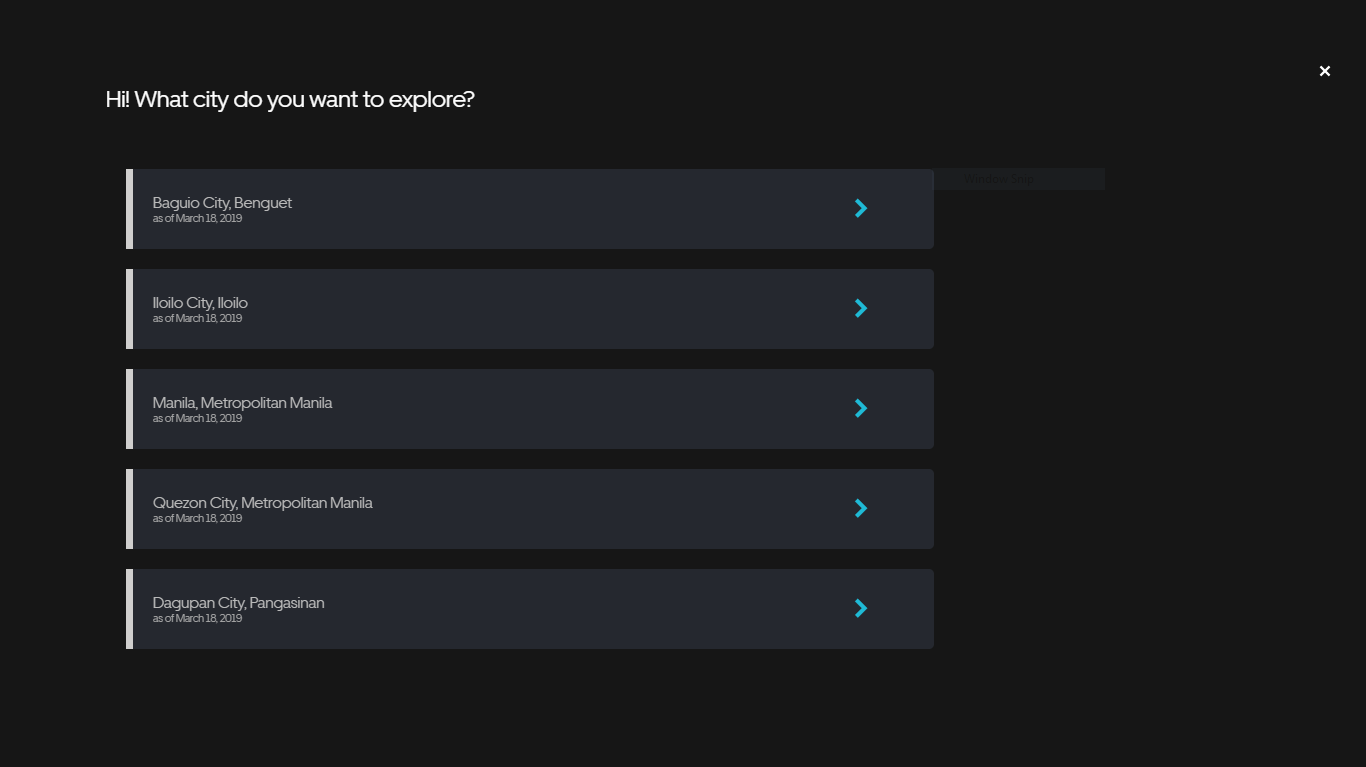
\includegraphics[width=0.9\columnwidth]{figures/kepler1.PNG}
  \caption{Initial view of Plexus where a user can choose what to view from the list of published cities }~\label{fig:KeplerCityList}
\end{figure}

\begin{figure}
\centering
  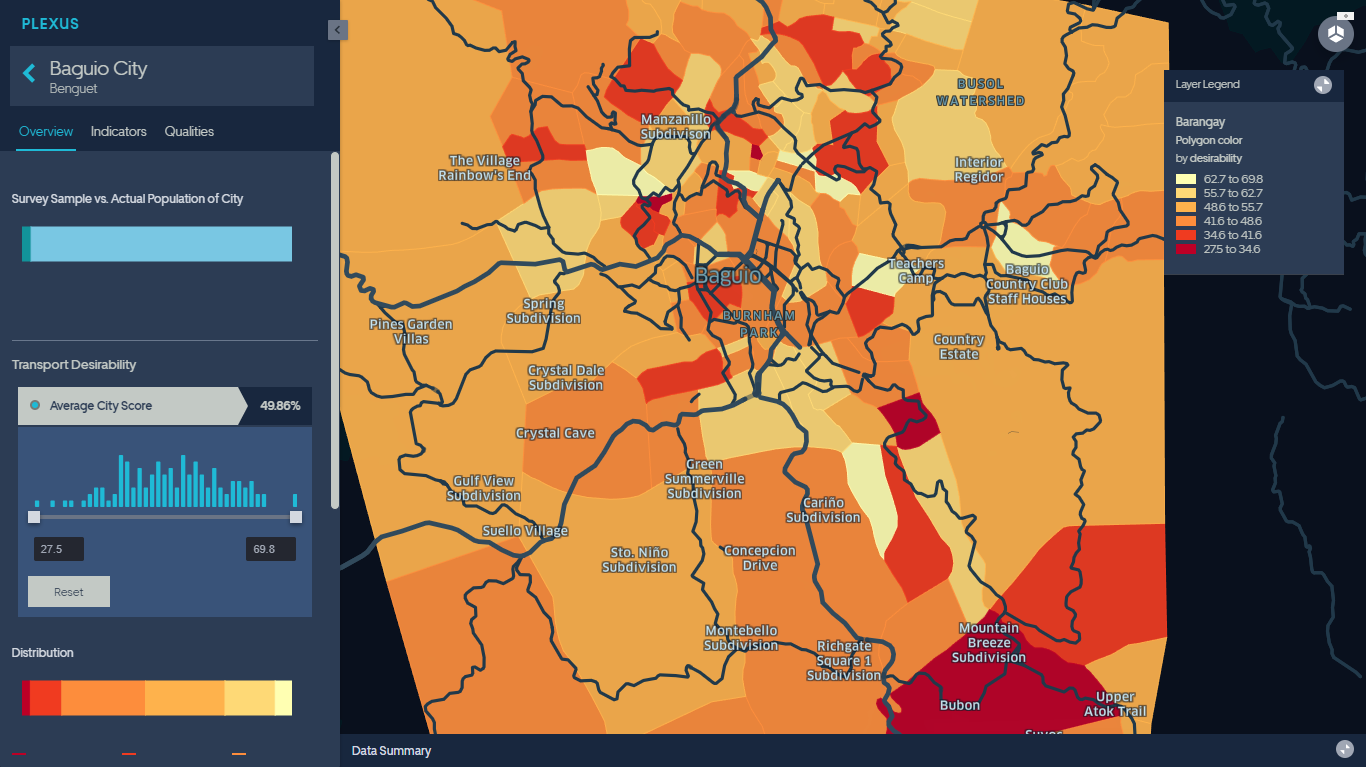
\includegraphics[width=0.9\columnwidth]{figures/overview.PNG}
  \caption{Overview of Plexus showing the overall city information in the left panel, and the choropleth map with its corresponding legend }~\label{fig:KeplerInitialView}
\end{figure}

An initially provided with a list of locations are accessible to the user. Before proceeding to the interactive map, the user may opt to select a location to be presented and assessed. Once a location is selected, the user will be presented with an interactive map and a visible left side panel. The interactive map could be interacted with using elements on the left side panel and interacting with the map itself. The map could be used for visualizing transport desirability-related scores and data.

\subsubsection{Techniques for Visualizing Transport Desirability-related Scores}
Each map view is separated by city based on the user’s choice and is overlaid by a choropleth map. It first displays the transport desirability score per barangay using a quantize color scale. As seen in Figure \ref{fig:KeplerInitialView}, the color scheme used ranged from light yellow for a high desirability and indicator score, to dark red for a low score. The color scheme initially used for the choropleth map ranged from light green to dark blue during UT1. However, it did not help in intuitively determining which areas need transport intervention for users, especially with UT1N. The colors that were chosen were predefined by Kepler.gl. Moreover, as red is the color for urgency and is eye-catching, it was used to color problem areas in the city. This was seen as more intuitive by UT2 participants. The legends for the colors are located in a collapsible panel on the upper right corner of the screen to guide users in interpreting the colors. In the initial stages of the system, the road network of the city was not included in the map view, but was later included since UT1 participants deemed this important for giving insights of the existing transport infrastructure a city or barangay.

\subsubsection{Techniques for Visualizing Other Related Data}
As presented in Figure \ref{fig:KeplerAmenities}, an icon map was used in visualizing amenities found in a city. The icons used were acquired from the Kepler.gl library. Each category for amenities were represented by different icons that are visually descriptive to make the icons discernible. Since we could not add or modify icons, we picked icons that had the nearest relation possible to the amenities. Aside from this, the colors were also initially dependent on the amenity category, but was visually overwhelming for UT1 participants, especially when all amenity categories were visible on the map. Although the ideal solution would be to add a circular background or pin to the icons, it could not be implemented. Due to this, all icons were colored white for a work around solution.


\begin{figure}
\centering
  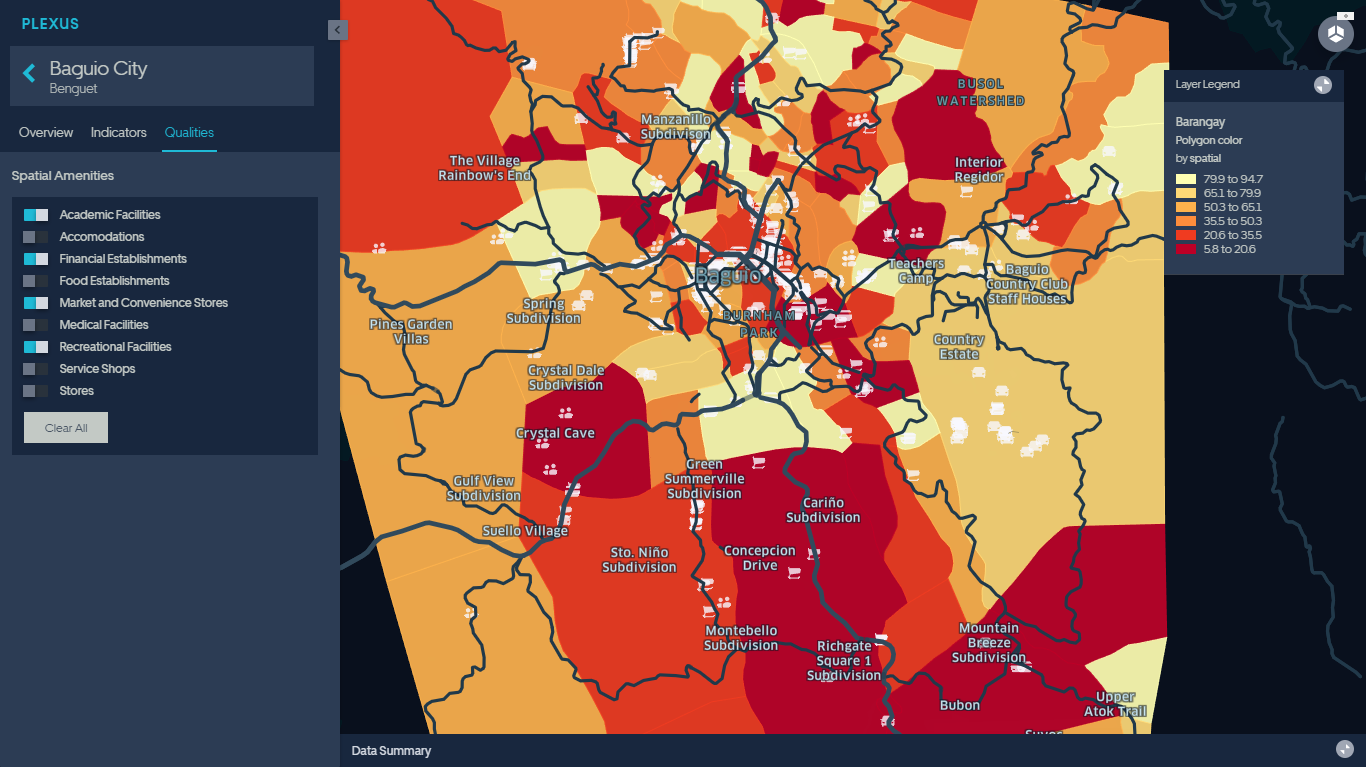
\includegraphics[width=0.9\columnwidth]{figures/kepler9.PNG}
  \caption{Academic facilities, financial establishments, market and convenience stores, and recreational facilities are made visible on the map using the left panel }~\label{fig:KeplerAmenities}
\end{figure}

The desire lines are displayed using a range of blues to contrast the colors in the choropleth map as shown in Figure \ref{fig:KeplerDesireLines} and represents the number of people going from a certain origin to a destination, with a darker blue signifying a larger amount of people. The initial implementation only displays arcs with no visible arrow to show its direction as Kepler.gl does not support arrowheads or textures for the arc visualizations. As a result, the frequent origin and destinations of the barangay are shown in the right panel when a barangay is clicked. The system also has an implemented 3D map view where arcs can be seen more clearly.

\begin{figure}
\centering
  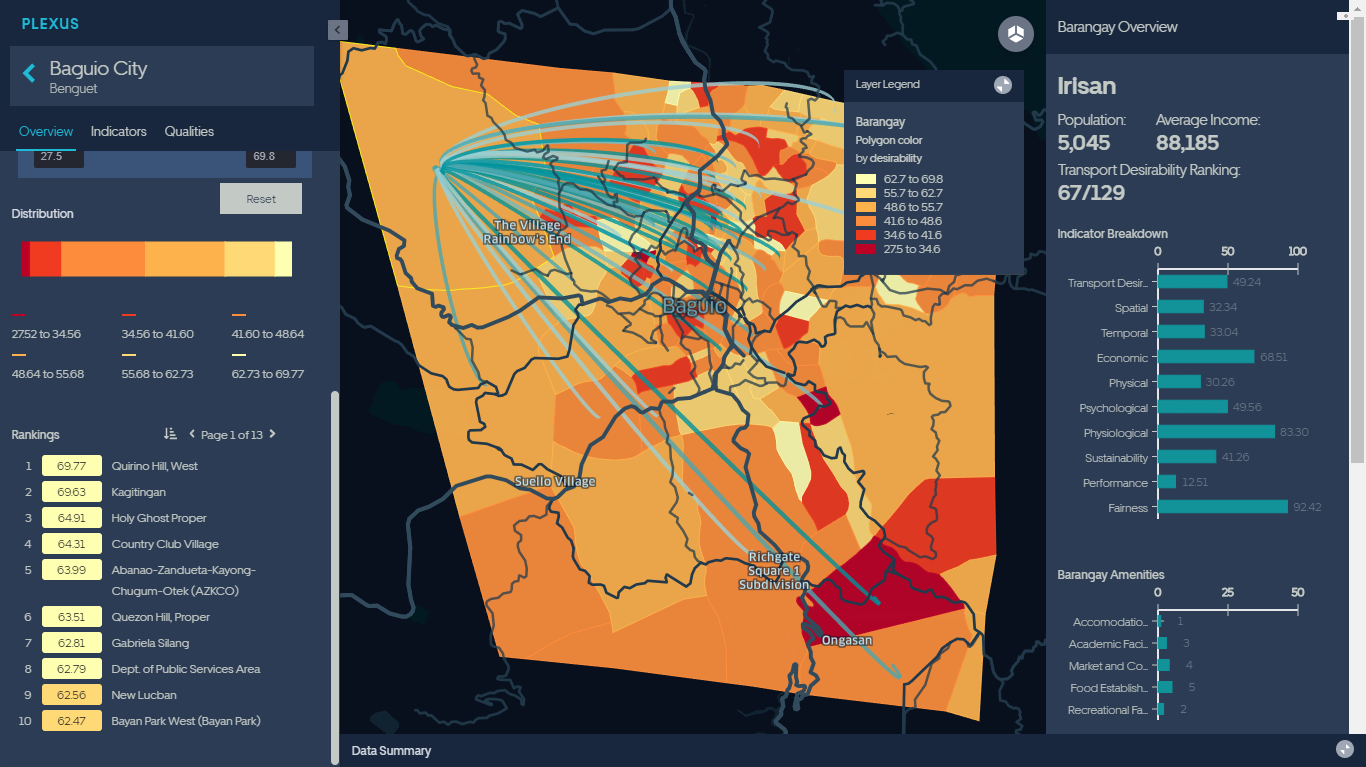
\includegraphics[width=0.9\columnwidth]{figures/overview2.PNG}
  \caption{Desire lines showing the barangay Irisan as the origin, its corresponding destinations, and an overview of the barangay in the right panel }~\label{fig:KeplerDesireLines}
\end{figure}

\subsubsection{Interactivity of Map}
The interactivity of the map allows the user to hover or click on a certain barangay. Once hovered, a tooltip will be shown to display the barangay name and its transport desirability score. When transport desirability-related scores are filtered, barangays that do not meet the criteria of the filter will be left with only their borders.  Lastly, when a barangay on the map has recorded origin-destination data and is clicked, its corresponding origin-destination desire lines will appear and shows the volume of commuters going from that path when hovered. Based from UT2 and UT3 participants, “Origin to destination” was a confusing header for the textbox, Therefore this was changed to “<Origin Barangay name> to <Destination Barangay name>” for the following test. A right side panel will also become visible and will be discussed in the next subsection.

\subsection{Investigating City and Barangay Data through Side Panels}
Non-geographical data, such as statistical visualization techniques and aggregated datasets, were also utilized in order to describe and give an overview of a city and barangay. Two panels were situated in both sides of the screen with different purposes.

The left side panel holds the city information. In Figure \ref{fig:KeplerInitialView}, it can be seen that the city name and region is printed at the top most of the panel. Below it are three tabs namely: \textit{Overview}, \textit{Indicators}, and \textit{Qualities}. The \textit{Overview} tab serves as a general overview of the city which contains the actual and sample population of the city, the ranking of barangays arranged from highest to lowest transport desirability score, the transport desirability score of the city, and the distribution of transport desirability scores within the city. The rankings if the barangays are color-coded similar to the map. Initially, the transport desirability score was included in the \textit{Indicator} tab, but it was moved due to the fact that it is an aggregated score of the indicators and is therefore, not actually a part of the indicators. Moreover, UT2N could not quickly find the transport desirability score of the city, leading to the decision to move it to the Overview tab. The \textit{Indicator} tab shows the indicator scores listed as buttons, with their corresponding score displayed at the right side. Clicking an indicator reflects on the choropleth map and shows a range filter as shown in Figure \ref{fig:KeplerIndicatorActive}. Each indicator was also provided a description and can be accessed by hovering on its corresponding button. These  were consulted with an expert on the transport desirability framework. Lastly, the \textit{Qualities} tab contains functions for amenities. A user can toggle the visibility of an amenity category on the map as seen in Figure \ref{fig:KeplerAmenities}.

%!!!!!!!!!!!!!!!!
\begin{figure}
\centering
  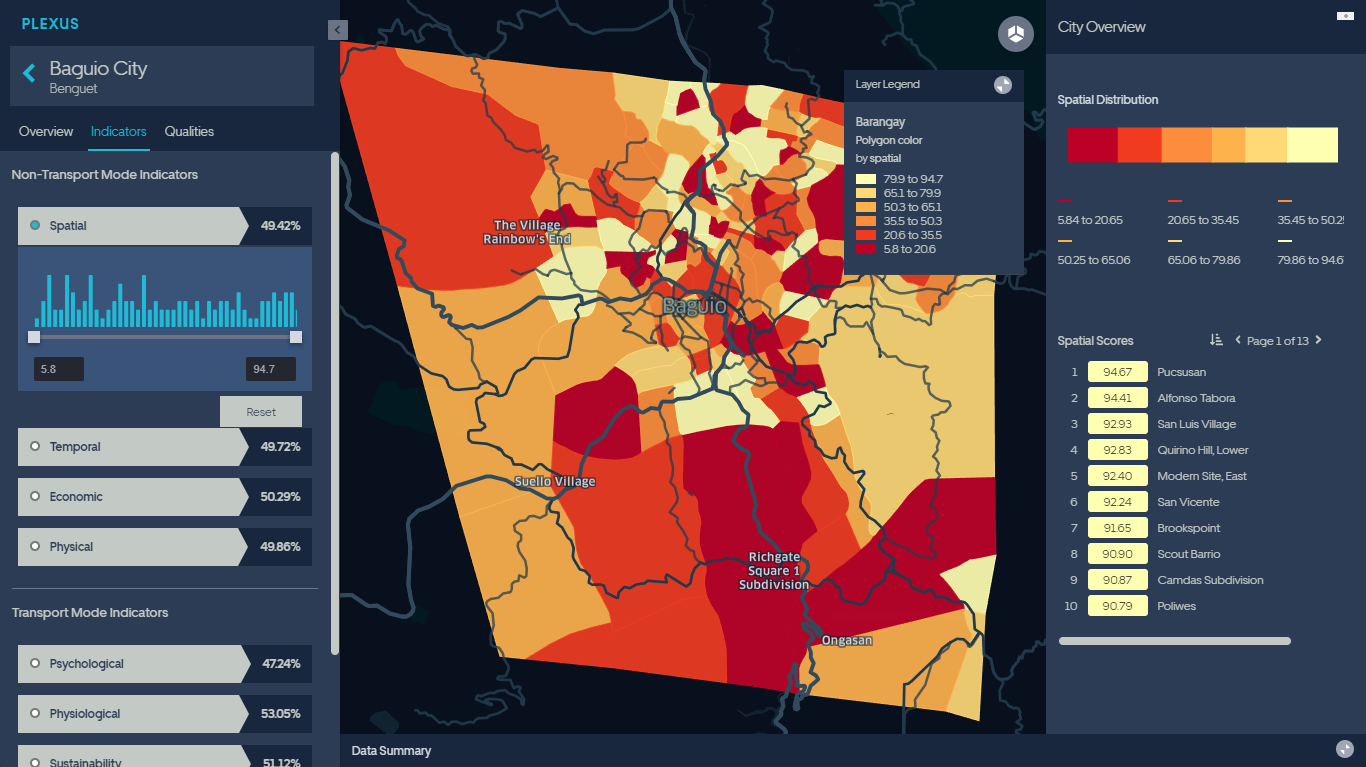
\includegraphics[width=0.9\columnwidth]{figures/indicator.PNG}
  \caption{A distribution and barangay ranking according to the spatial amenity is shown on the right panel}~\label{fig:KeplerIndicatorActive}
\end{figure}

The right panel displays if either an indicator is selected on the right panel or if a barangay is selected on the map. When an indicator is selected, the distribution of the indicator scores in a quantize color scale are presented in a stacked bar chart, and the rankings of all barangays according to the selected indicator are shown, as seen in Figure \ref{fig:KeplerIndicatorActive}. When a barangay is clicked, shown in Figure \ref{fig:KeplerDesireLines} only the barangay information is shown. This was done to segregate the purpose of the panels. The name, population, average income, and the ranking of the barangay according to the selected indicator or transport desirability are positioned at the topmost part of the panel. Aside from this, a bar graph displaying the breakdown of the barangay’s indicator scores are also positioned in this panel to supply an overview of its current state of transportation. A bar graph was used instead of multiple pie charts for indicators to conserve space and to compare the scores of an indicator to other indicators.

\begin{figure}
\centering
  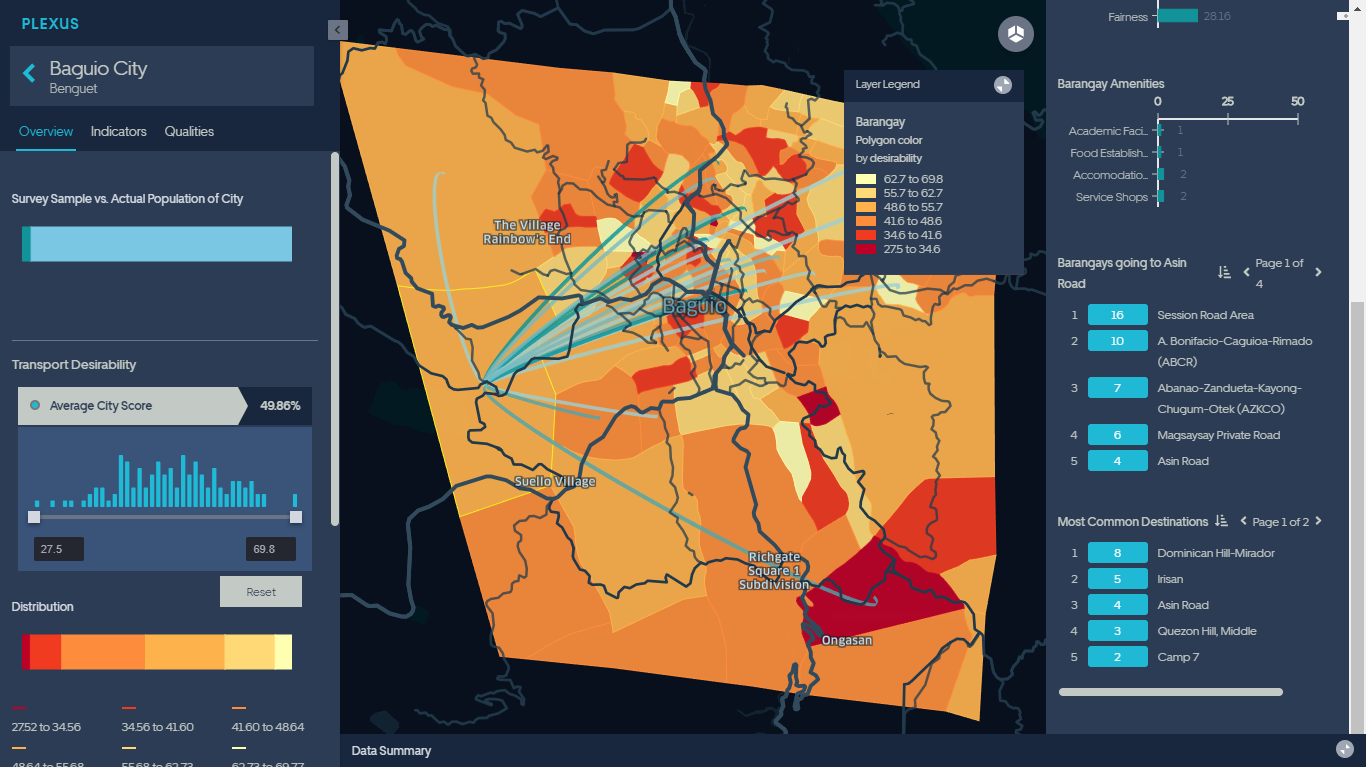
\includegraphics[width=0.9\columnwidth]{figures/overview-barangay-2.PNG}
  \caption{Occurring origins and frequent destination of Asin Road situated in the right panel}~\label{fig:KeplerBarangayContd}
\end{figure}

\subsection{Assessing Multivariate Data using Data Stories}
The data stories are located in the bottom panel in the screen and it intends to present a visualized overview of the state of indicators throughout all barangays in the city.

\subsubsection{Parallel Coordinates and Table View of Data}
The parallel coordinates hold the indicators as the items in the x-axis and the barangays as the lines, as illustrated in Figure \ref{fig:KeplerParallelCoords}. In comparison to the visualization techniques presented in the previous section, these coordinates and tables are more catered to showing trends in the indicator scores and can be used in comparing the scores of multiple barangays at once. It can be filtered using the transport desirability and indicator range filters in the left panel. The colors used in the parallel coordinates are similar to the colors presented in the choropleth map to immediately form a darker shade in the instance of multiple barangays having the same values or trends. The table will only show the data selected in the parallel coordinates, and all data will be shown if this does not apply. In the table, the columns presented are the barangay name, average income, population, transport desirability score, and their corresponding indicator scores and can be sorted in either ascending or descending order. During UT2 and UT3, most participants were confused with the interactivity of the parallel coordinates. Therefore, we modified the sorting function to be activated through the table column names instead.

\begin{figure}
\centering
  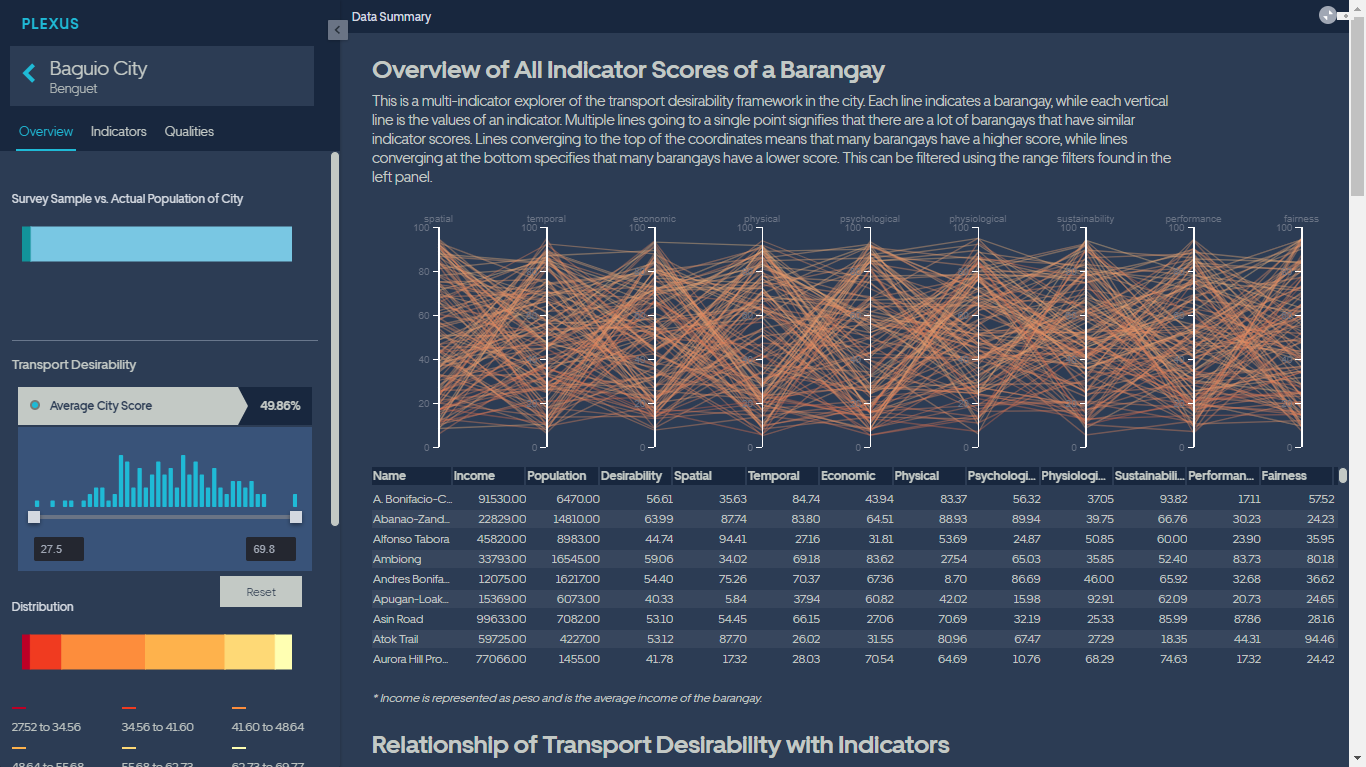
\includegraphics[width=0.9\columnwidth]{figures/overview-dsum.PNG}
  \caption{Parallel coordinates and its corresponding data in table view showing the indicators of the barangays}~\label{fig:KeplerParallelCoords}
\end{figure}


\subsubsection{Comparison of Transport Desirability and Indicator Score}
As seen in Figure \ref{fig:KeplerScatterPlot}, scatter plots were utilized in order to show a correlation between the transport desirability score and indicator score. This was done to give the user a bi-variate view of data that could help in defining which indicators greatly affect the city’s overall transport desirability.

\begin{figure}
\centering
  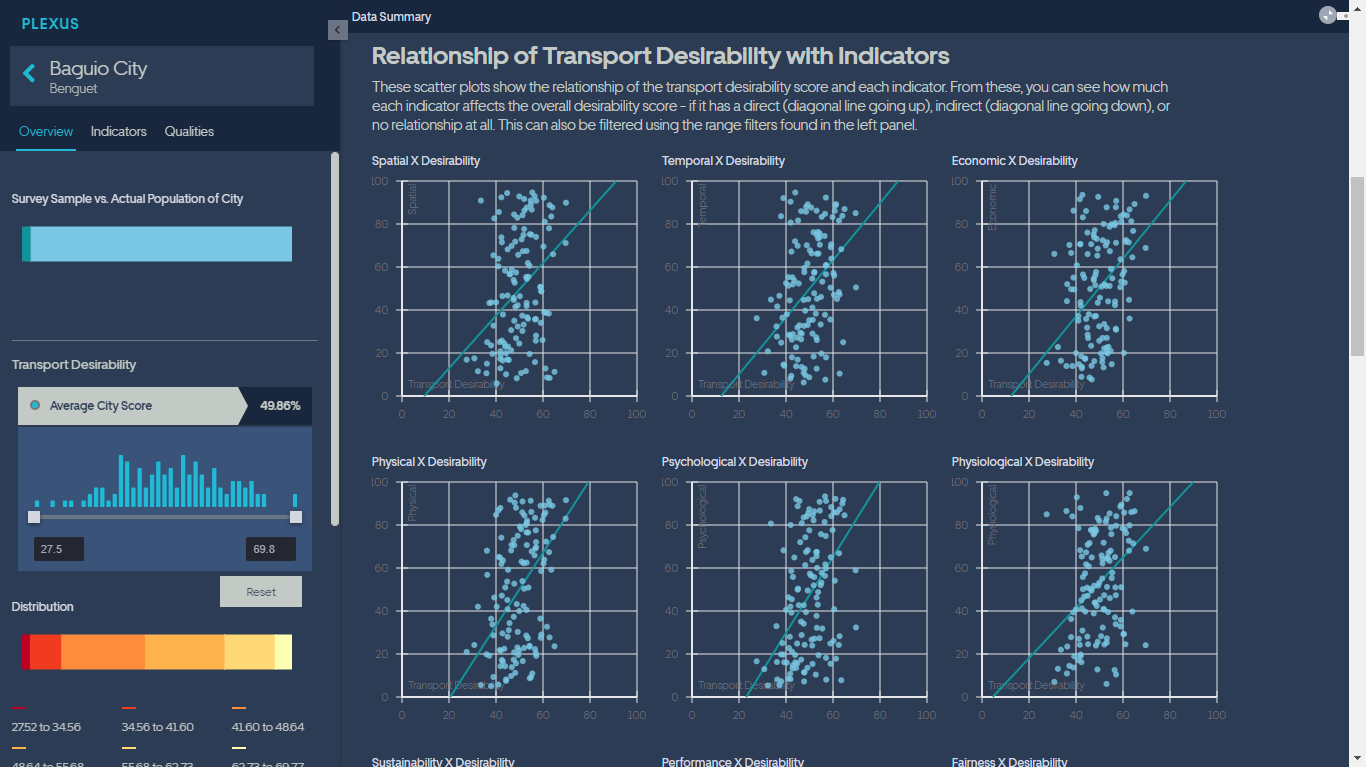
\includegraphics[width=0.9\columnwidth]{figures/overview-dsplot.PNG}
  \caption{Scatter plots showing the relationship of all indicators and the transport desirability score}~\label{fig:KeplerScatterPlot}
\end{figure}

\subsubsection{City Amenities and Frequented Destinations}
A summary of city amenities are presented by category and their corresponding count. Furthermore, the frequent destinations in the city, separated by mode share are also displayed. These information are shown as bar charts and stacked bar charts, respectively. Frequent destinations are sorted in descending order depending on the number of people traveling to that certain barangay, as shown in Figure \ref{fig:KeplerAmenitiyModeShare}.

\begin{figure}
\centering
  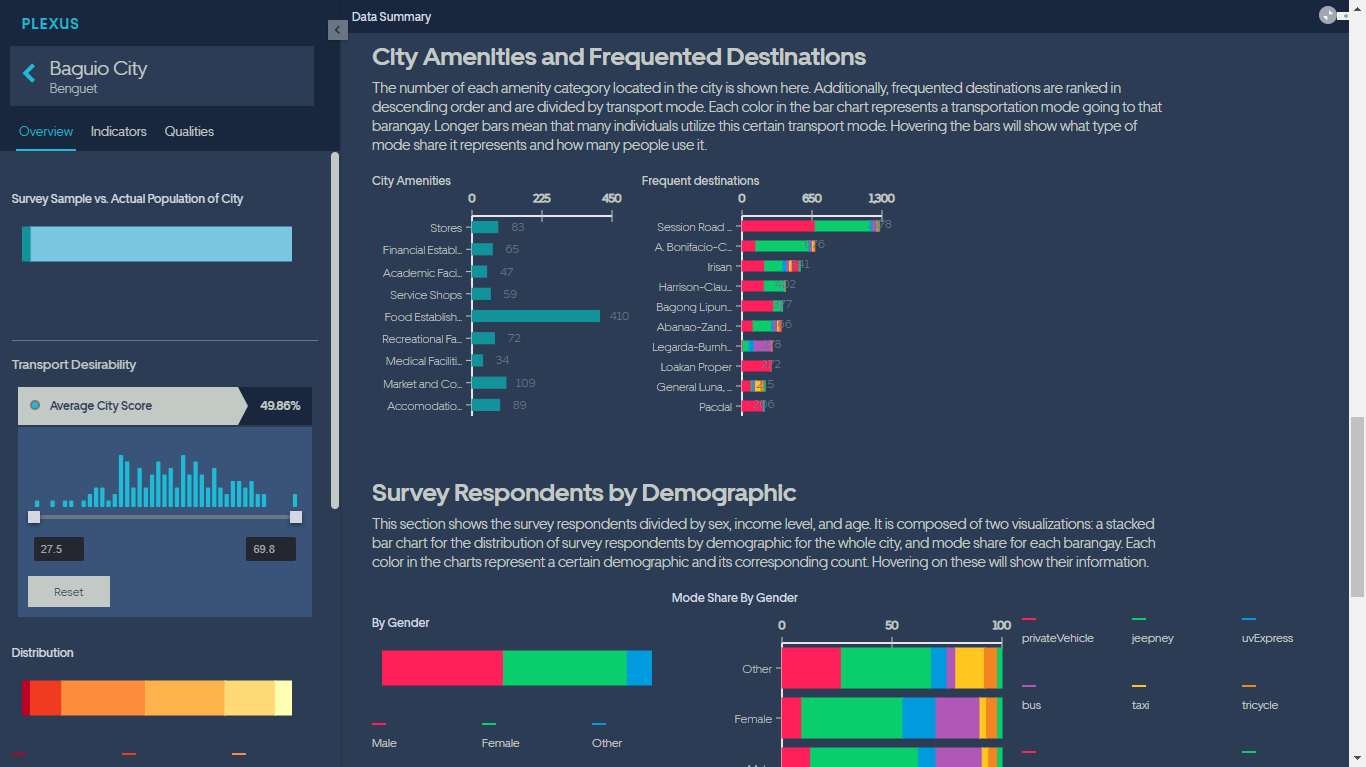
\includegraphics[width=0.9\columnwidth]{figures/overview-dscityam.PNG}
  \caption{City amenities bar chart showing the number of amenities per category, and the frequent destinations bar chart showing the list of frequented barangays partitioned by mode share}~\label{fig:KeplerAmenitiyModeShare}
\end{figure}

\subsubsection{Survey Data Share by Demographic}
The mode share and demographics from the sample population that was surveyed can be classified by sex, income level, and age. These are then separated by barangay, and can be helpful in canvassing factors that could have an effect in transportation behavior. These factors are represented through a stacked bar chart to see its distribution in both the city and the barangay. This can be seen in Figure \ref{fig:KeplerSurveyShare}.

\begin{figure}
\centering
  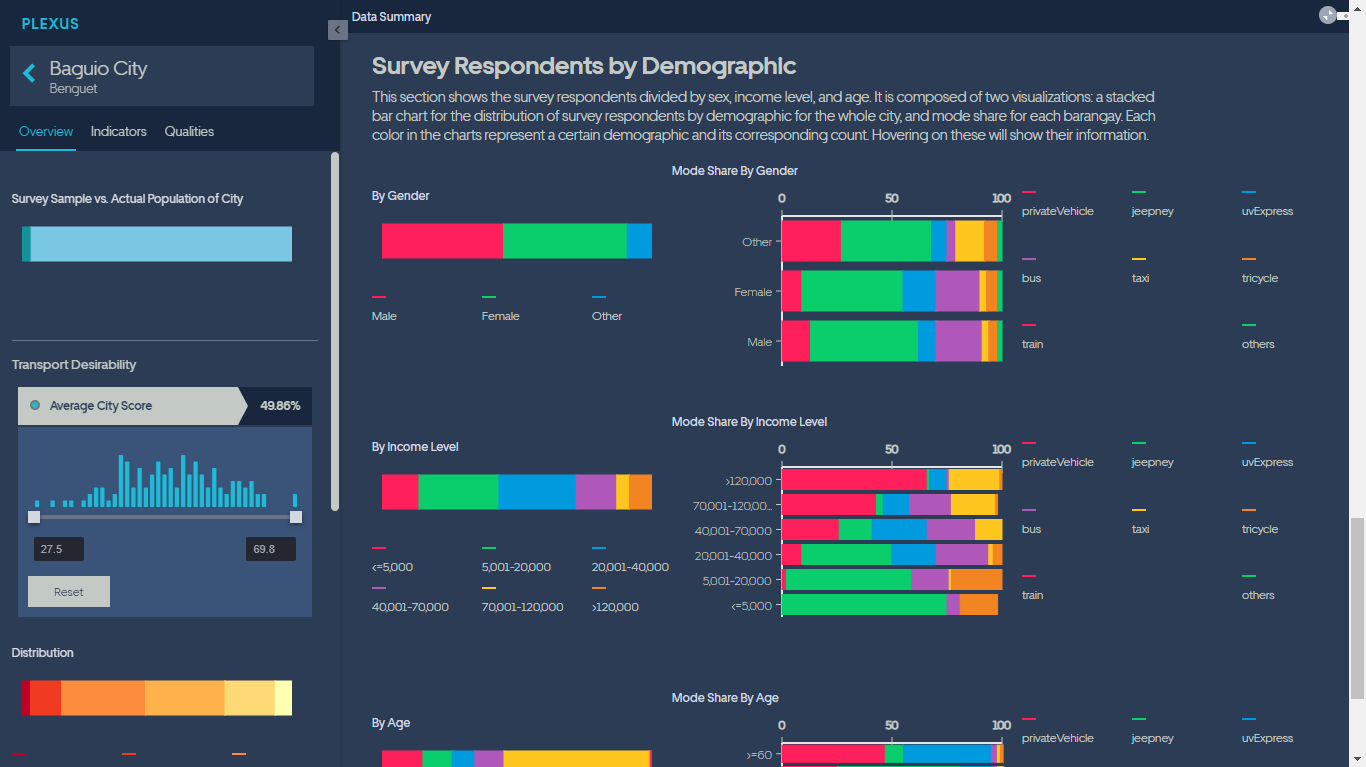
\includegraphics[width=0.9\columnwidth]{figures/overview-dsdemo.PNG}
  \caption{Visualization of mode share and demographics in the city organized by sex, income level, and age}~\label{fig:KeplerSurveyShare}
\end{figure}

\section{Experimental Design}
For the experiment that will be conducted, nine novices will create transport desirability assessments based on given tasks. However, these novices will be divided into three groups; Each group will be utilizing a different tool for their assessment. The first group (G1), the second group (G2), and the third group (G3) will be utilizing spreadsheet applications, Plexus without data stories, and Plexus with data stories respectively. After each task, each participant will be required to answer a NASA-TLX questionnaire to quantify the mental workload endured for each task. Moreover, each participant will be asked about their experience doing the task to qualitatively determine the system’s usability.  

For result analysis, experts in transport desirability assessment will be rating the resulting assessments of novices depending on their process and their output. The ratings will be on a scale of 1 to 7, with 7 being excellent and 1 being highly unsatisfactory. Both expert ratings and NASA-TLX results will be used to compare the different groups and to check if data stories positively affected the quality of assessments.  

\section{Discussion}
The designs of the interactions were developed and repeatedly improved through three iterations. Initially, Plexus was designed only to show transport desirability, its indicators and qualities, and the locations of the barangay. From design critiques and usability tests, it was shown that the initial features were not enough to create an assessment as assumptions could not be verified through the system. This led to adding road networks, data visualizations for summarization, and filtering. Moreover, more information of the origins going to a barangay, the destinations from a barangay, a barangay’s amenities, population, and average income were shown when a barangay was clicked. Rankings were also provided to the user to instantly pinpoint barangays that require prioritization in a transport plan. Information was also segregated into panels, which was greatly improved through design critiques and usability tests. For the second usability test, it was clear for most participants that the left panel was for city information, the right panel was for barangay information, and the bottom panel was for summaries. From the fourth iteration, it was also observed that the lack of knowledge on transport desirability could have affected the assessment of novices during the second iteration. Although new participants tested the application, they had lower scores compared to new novices. This could be due to the participants in the third iteration had expertise in transport engineering. However, it was also observed that familiar novices also had similar performance and effort scores with new experts, showing that a novice could attain an expert assessment.

As data is dependent on a separate group of the project, Plexus only uses available data for transport desirability qualities. However, some data visualized in the system are still randomly generated. The origin-destination data is assumed to be one-way per individual surveyed, and only covers barangay to barangay travel. Therefore, origin-destination data involving different cities or regions, or origin-destination within one barangay only are not included, and only one city can be viewed at a time.

The system only visualizes the indicators and qualities included in the transport desirability framework. However, not all qualities are included since some data required for these are lacking. Furthermore, connectivity, orderliness, and service reliability data are not visualized in the system. Computed indicator scores and transport desirability scores, household information, and trip information will be accessible in the database through the admin console. Furthermore, survey data visualized in the system will also be obtained beforehand, thus the system does not reflect real-time data.

\section{Conclusion and Future Work}
This study employs a participatory design methodology in developing the system. In the early stages of development, co-design sessions were employed to refine information architecture, and to identify visualizations and workflow for the system. To iteratively improve the usability of the system, four usability tests were done with novices and experts. Overall, the resulting features were an interactive map, a side panel for city information and map controls, a side panel for supporting data of barangay and city indicators, and a bottom panel for data stories. From these tests, the system was deemed usable by novices and experts, as general mental workload decreased and confidence rating increased. However, the transferring of expert knowledge to novices was not focused in previous usability tests. Therefore, for the next experiment, we aim to focus on determining the effect of data stories on assessments.

The current application could still be improved in terms of features and data. Data visualizations such as icons and origin-destination desire lines could be improved by modifying their shape, yet was not done for this study as it is a technical limitation of Kepler.gl, a system that Plexus is extended from. Moreover, base map designs for terrain and satellite views were not utilized, yet were deemed useful by some participants for decisions related to road construction.

As mentioned in design critiques, traffic data per day and time would be helpful for users to decide on routes. However, due to the lack of this data for this study, it was not implemented. Also, useful information per indicator was not fully implemented in the system due to the framework still being developed. Moreover, more information on mode share and trips should be added to allow for deeper assessments.

As experts deemed non-expert assessments to be fairly acceptable with scores ranging from 4 to 6 out of 7, it could still be improved. Therefore, more consultations with transport desirability assessment experts would be needed to improve data summaries for non-experts to acquire expert-like assessments. An experiment on the effect of a refined data summary could also be done to observe if data summaries could affect the assessment quality of non-experts.

As the Philippines lacks experts in transport engineering, it was difficult to invite more experts to test the system and to recommend features and useful data. Inviting transport engineers and researchers from private firms could lead to a greater perspective for the system’s design and interactions. More iterations would be ideal to improve more on information architecture and interactions within the system.  











% \subsection{References and Citations}

% Use a numbered list of references at the end of the article, ordered
% alphabetically by last name of first author, and referenced by numbers
% in
% brackets~\cite{acm_categories,ethics,Klemmer:2002:WSC:503376.503378}.
% Your references should be published materials accessible to the
% public. Internal technical reports may be cited only if they are
% easily accessible (i.e., you provide the address for obtaining the
% report within your citation) and may be obtained by any reader for a
% nominal fee. Proprietary information may not be cited. Private
% communications should be acknowledged in the main text, not referenced
% (e.g., ``[Borriello, personal communication]'').

% References should be in ACM citation format:
% \url{http://acm.org/publications/submissions/latex_style}. This
% includes citations to internet
% resources~\cite{acm_categories,cavender:writing,CHINOSAUR:venue,psy:gangnam}
% according to ACM format, although it is often appropriate to include
% URLs directly in the text, as above.


% % Use a numbered list of references at the end of the article, ordered
% % alphabetically by first author, and referenced by numbers in
% % brackets~\cite{ethics, Klemmer:2002:WSC:503376.503378,
% %   Mather:2000:MUT, Zellweger:2001:FAO:504216.504224}. For papers from
% % conference proceedings, include the title of the paper and an
% % abbreviated name of the conference (e.g., for Interact 2003
% % proceedings, use \textit{Proc. Interact 2003}). Do not include the
% % location of the conference or the exact date; do include the page
% % numbers if available. See the examples of citations at the end of this
% % document. Within this template file, use the \texttt{References} style
% % for the text of your citation.

% % Your references should be published materials accessible to the
% % public.  Internal technical reports may be cited only if they are
% % easily accessible (i.e., you provide the address for obtaining the
% % report within your citation) and may be obtained by any reader for a
% % nominal fee.  Proprietary information may not be cited. Private
% % communications should be acknowledged in the main text, not referenced
% % (e.g., ``[Robertson, personal communication]'').

% \begin{table}
%   \centering
%   \begin{tabular}{l r r r}
%     % \toprule
%     & & \multicolumn{2}{c}{\small{\textbf{Test Conditions}}} \\
%     \cmidrule(r){3-4}
%     {\small\textit{Name}}
%     & {\small \textit{First}}
%       & {\small \textit{Second}}
%     & {\small \textit{Final}} \\
%     \midrule
%     Marsden & 223.0 & 44 & 432,321 \\
%     Nass & 22.2 & 16 & 234,333 \\
%     Borriello & 22.9 & 11 & 93,123 \\
%     Karat & 34.9 & 2200 & 103,322 \\
%     % \bottomrule
%   \end{tabular}
%   \caption{Table captions should be placed below the table. We
%     recommend table lines be 1 point, 25\% black. Minimize use of
%     table grid lines.}~\label{tab:table1}
% \end{table}

% \section{Sections}

% The heading of a section should be in Helvetica or Arial 9-point bold,
% all in capitals. Sections should \textit{not} be numbered.

% \subsection{Subsections}

% Headings of subsections should be in Helvetica or Arial 9-point bold
% with initial letters capitalized.  For sub-sections and
% sub-subsections, a word like \emph{the} or \emph{of} is not
% capitalized unless it is the first word of the heading.

% \subsubsection{Sub-subsections}

% Headings for sub-subsections should be in Helvetica or Arial 9-point
% italic with initial letters capitalized.  Standard
% \texttt{{\textbackslash}section}, \texttt{{\textbackslash}subsection},
% and \texttt{{\textbackslash}subsubsection} commands will work fine in
% this template.

% \section{Figures/Captions}

% Place figures and tables at the top or bottom of the appropriate
% column or columns, on the same page as the relevant text (see
% Figure~\ref{fig:figure1}). A figure or table may extend across both
% columns to a maximum width of 17.78 cm (7 in.).

% \begin{figure*}
%   \centering
%   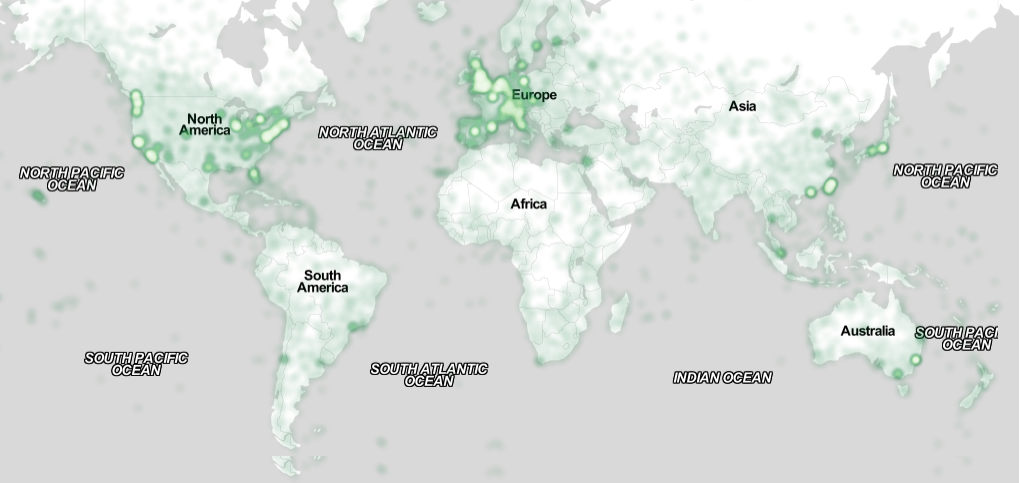
\includegraphics[width=1.75\columnwidth]{figures/map}
%   \caption{In this image, the map maximizes use of space. You can make
%     figures as wide as you need, up to a maximum of the full width of
%     both columns. Note that \LaTeX\ tends to render large figures on a
%     dedicated page. Image: \ccbynd~ayman on
%     Flickr.}~\label{fig:figure2}
% \end{figure*}

% Captions should be Times New Roman or Times Roman 9-point bold.  They
% should be numbered (e.g., ``Table~\ref{tab:table1}'' or
% ``Figure~\ref{fig:figure1}''), centered (if one line) otherwise justified, and placed beneath the figure
% or table.  Please note that the words ``Figure'' and ``Table'' should
% be spelled out (e.g., ``Figure'' rather than ``Fig.'') wherever they
% occur. Figures, like Figure~\ref{fig:figure2}, may span columns and
% all figures should also include alt text for improved accessibility.
% Papers and notes may use color figures, which are included in the page
% limit; the figures must be usable when printed in black-and-white in
% the proceedings.

% The paper may be accompanied by a short video figure (we recommend staying within five
% minutes in length). However, the paper should stand on its own without
% the video figure, as the video may not be available to everyone who
% reads the paper.  

% \subsection{Inserting Images}
% When possible, include a vector formatted graphic (i.e. PDF or EPS).
% When including bitmaps,  use an image editing tool to resize the image
% at the appropriate printing resolution (usually 300 dpi).

% \section{Quotations}
% Quotations may be italicized when \textit{``placed inline''}.

% \begin{quote}
% Longer quotes, when placed in their own paragraph, need not be
% italicized or in quotation marks when indented.  
% \end{quote}

% \section{Language, Style, and Content}

% The written and spoken language of SIGCHI is English. Spelling and
% punctuation may use any dialect of English (e.g., British, Canadian,
% US, etc.) provided this is done consis- tently. Hyphenation is
% optional. To ensure suitability for an international audience, please
% pay attention to the following:

% \begin{itemize}
% \item Write in a straightforward style.
% \item Try to avoid long or complex sentence structures.
% \item Use common and basic vocabulary (e.g., use the word ``unusual'' rather than the word ``arcane''.
% \item Briefly define or explain all technical terms that may be
%   unfamiliar to readers.
% \item Explain all acronyms the first time they are used in your
%   text---e.g., ``Digital Signal Processing (DSP)''.
% \item Explain local references (e.g., not everyone knows all city
%   names in a particular country).
% \item Explain ``insider'' comments. Ensure that your whole audience
%   understands any reference whose meaning you do not describe (e.g.,
%   do not assume that everyone has used a Macintosh or a particular
%   application).
% \item Explain colloquial language and puns. Understanding phrases like
%   ``red herring'' may require a local knowledge of English.  Humor and
%   irony are difficult to translate.
% \item Use unambiguous forms for culturally localized concepts, such as
%   times, dates, currencies, and numbers (e.g., ``1--5--97'' or
%   ``5/1/97'' may mean 5 January or 1 May, and ``seven o'clock'' may
%   mean 7:00 am or 19:00). For currencies, indicate equivalences:
%   ``Participants were paid {\fontfamily{txr}\selectfont \textwon}
%   25,000, or roughly US \$22.''
% \item Be careful with the use of gender-specific pronouns (he, she)
%   and other gendered words (chairman, manpower, man-months). Use
%   inclusive language that is gender-neutral (e.g., she or he, they,
%   s/he, chair, staff, staff-hours, person-years). See the
%   \textit{Guidelines for Bias-Free Writing} for further advice and
%   examples regarding gender and other personal
%   attributes~\cite{Schwartz:1995:GBF}. Be particularly aware of
%   considerations around writing about people with disabilities.
% \item If possible, use the full (extended) alphabetic character set
%   for names of persons, institutions, and places (e.g.,
%   Gr{\o}nb{\ae}k, Lafreni\'ere, S\'anchez, Nguy{\~{\^{e}}}n,
%   Universit{\"a}t, Wei{\ss}enbach, Z{\"u}llighoven, \r{A}rhus, etc.).
%   These characters are already included in most versions and variants
%   of Times, Helvetica, and Arial fonts.
% \end{itemize}

% \section{Accessibility}
% The Executive Council of SIGCHI has committed to making SIGCHI
% conferences more inclusive for researchers, practitioners, and
% educators with disabilities. As a part of this goal, the all authors
% are asked to work on improving the accessibility of their
% submissions. Specifically, we encourage authors to carry out the
% following five steps:
% \begin{enumerate}
% \item Add alternative text to all figures
% \item Mark table headings
% \item Add tags to the PDF
% \item Verify the default language
% \item Set the tab order to ``Use Document Structure''
% \end{enumerate}
% For more information and links to instructions and resources, please
% see: \url{http://chi2016.acm.org/accessibility}.  The
% \texttt{{\textbackslash}hyperref} package allows you to create well tagged PDF files,
% please see the preamble of this template for an example.

% \section{Page Numbering, Headers and Footers}
% Your final submission should not contain footer or header information
% at the top or bottom of each page. Specifically, your final submission
% should not include page numbers. Initial submissions may include page
% numbers, but these must be removed for camera-ready. Page numbers will
% be added to the PDF when the proceedings are assembled.

% \section{Producing and Testing PDF Files}

% We recommend that you produce a PDF version of your submission well
% before the final deadline.  Your PDF file must be ACM DL
% Compliant. The requirements for an ACM Compliant PDF are available at:
% {\url{http://www.scomminc.com/pp/acmsig/ACM-DL-pdfs-requirements.htm}}.

% Test your PDF file by viewing or printing it with the same software we
% will use when we receive it, Adobe Acrobat Reader Version 10. This is
% widely available at no cost. Note that most
% reviewers will use a North American/European version of Acrobat
% reader, so please check your PDF accordingly.

% \section{Conclusion}

% It is important that you write for the SIGCHI audience. Please read
% previous years' proceedings to understand the writing style and
% conventions that successful authors have used. It is particularly
% important that you state clearly what you have done, not merely what
% you plan to do, and explain how your work is different from previously
% published work, i.e., the unique contribution that your work makes to
% the field. Please consider what the reader will learn from your
% submission, and how they will find your work useful. If you write with
% these questions in mind, your work is more likely to be successful,
% both in being accepted into the conference, and in influencing the
% work of our field.

\section{Acknowledgments}

The authors would like to thank their advisers, Dr. Rafael Cabredo and Mr. Briane Paul Samson, and their panelists, Ms. Courtney Ngo and Ms. Jennifer Ureta, for offering their guidance and constructive comments that would help in improving the study. The authors would also like to thank the Commission on Higher Education (CHED) for the overall support in performing this study. Furthermore, they would also like to extend their gratitude to the principal investigator of the project, Dr. Jose Bienvenido Manuel Biona, as well as the co-investigators , Dr. Neil Stephen Lopez and Dr. Alexis Fillone, for sharing their expertise with regards to the field of transport desirability. Lastly, the authors would like to thank the participants in the usability testings for giving them fruitful insights that would greatly help in the objective of the study.

% Balancing columns in a ref list is a bit of a pain because you
% either use a hack like flushend or balance, or manually insert
% a column break.  http://www.tex.ac.uk/cgi-bin/texfaq2html?label=balance
% multicols doesn't work because we're already in two-column mode,
% and flushend isn't awesome, so I choose balance.  See this
% for more info: http://cs.brown.edu/system/software/latex/doc/balance.pdf
%
% Note that in a perfect world balance wants to be in the first
% column of the last page.
%
% If balance doesn't work for you, you can remove that and
% hard-code a column break into the bbl file right before you
% submit:
%
% http://stackoverflow.com/questions/2149854/how-to-manually-equalize-columns-
% in-an-ieee-paper-if-using-bibtex
%
% Or, just remove \balance and give up on balancing the last page.
%
\balance{}

% \section{References Format}
% Your references should be published materials accessible to the
% public. Internal technical reports may be cited only if they are
% easily accessible and may be obtained by any reader for a nominal
% fee. Proprietary information may not be cited. Private communications
% should be acknowledged in the main text, not referenced (e.g.,
% [Golovchinsky, personal communication]). References must be the same
% font size as other body text. References should be in alphabetical
% order by last name of first author. Use a numbered list of references
% at the end of the article, ordered alphabetically by last name of
% first author, and referenced by numbers in brackets. For papers from
% conference proceedings, include the title of the paper and the name of
% the conference. Do not include the location of the conference or the
% exact date; do include the page numbers if available. 

% References should be in ACM citation format:
% \url{http://www.acm.org/publications/submissions/latex_style}.  This
% includes citations to Internet
% resources~\cite{CHINOSAUR:venue,cavender:writing,psy:gangnam}
% according to ACM format, although it is often appropriate to include
% URLs directly in the text, as above. Example reference formatting for
% individual journal articles~\cite{ethics}, articles in conference
% proceedings~\cite{Klemmer:2002:WSC:503376.503378},
% books~\cite{Schwartz:1995:GBF}, theses~\cite{sutherland:sketchpad},
% book chapters~\cite{winner:politics}, an entire journal
% issue~\cite{kaye:puc},
% websites~\cite{acm_categories,cavender:writing},
% tweets~\cite{CHINOSAUR:venue}, patents~\cite{heilig:sensorama}, 
% games~\cite{supermetroid:snes}, and
% online videos~\cite{psy:gangnam} is given here.  See the examples of
% citations at the end of this document and in the accompanying
% \texttt{BibTeX} document. This formatting is a edited version of the
% format automatically generated by the ACM Digital Library
% (\url{http://dl.acm.org}) as ``ACM Ref.'' DOI and/or URL links are
% optional but encouraged as are full first names. Note that the
% Hyperlink style used throughout this document uses blue links;
% however, URLs in the references section may optionally appear in
% black.

% BALANCE COLUMNS
\balance{}

% REFERENCES FORMAT
% References must be the same font size as other body text.
\bibliographystyle{SIGCHI-Reference-Format}
\bibliography{sample}

\end{document}

%%% Local Variables:
%%% mode: latex
%%% TeX-master: t
%%% End:
